\subsection{Forma del fascio}

Abbiamo fatto delle misure di conteggio a vari angoli con e senza collimatori per studiare la forma del fascio.

\subsubsection{Assenza di collimatori}

La misura in assenza di collimatori ci permette di indagare la forma del fascio di particelle $\alpha$ in uscita dalla sorgente di \am{}.
\marginpar{disegno provvisorio}
Bisogna notare che l'angolo segnato sulla scala graduata non coincide con quello tra la sorgente ed il rivelatore perché il fotodiodo non è al centro della camera a vuoto, inoltre all'aumentare (in modulo) dell'angolo la distanza tra sorgente e rivelatore diminuisce. 
Lo schema di \autoref{fma} illustra la situazione.

\begin{figure}[h]
\centering
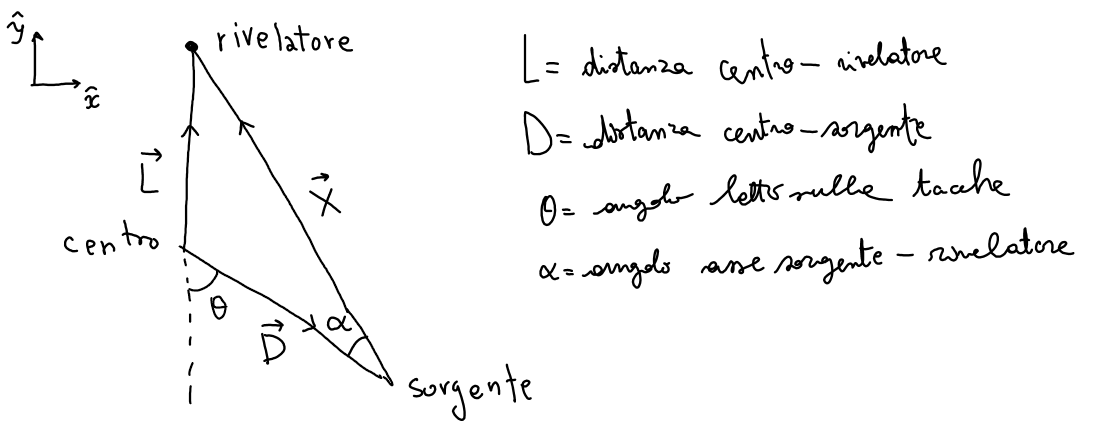
\includegraphics[width=30 em]{immagini/fma_provv}
\caption{Schema raffigurante gli angoli tra rivelatore, centro della camera a vuoto e sorgente.}
\label{fma}
\end{figure}

Applicate le dovute correzioni e usando le variabili di \autoref{fma} troviamo che l'angolo tra rivelatore e sorgente è
\begin{equation}
\cos{\alpha}= -\frac{\vec{X} \cdot \vec{D} }{ |\vec{X}| |\vec{D}| } = \frac{ L \cos{\theta} + D }{ \sqrt{ L^2+2LD\cos{\theta}+D^2  } }.
\end{equation}

Teniamo conto della variazione della distanza al variare dell'angolo moltiplicando ogni rate per $|\vec{X}|^2$.
Tale fattore è giustificato dal fatto che supponiamo isotropa l'emissione di particelle $\alpha$ da parte della sorgente.
Se $C$ è una costante, abbiamo che $$ \frac{dN}{d^3r}=C \implies \frac{dN}{dr}=C 4\pi r^2. $$

In virtù delle precedenti affermazioni, abbiamo calcolato il rate in \si{s^{-1}cm^2}.

Il risultato di questa misura è presente in \autoref{fig:forma}, invece la \autoref{tab:forma} contiene i dati di tale grafico.
Si evince che il fascio ha un'estensione angolare di quasi \SI{50}{\degree}. 

\begin{figure}[h]
\centering
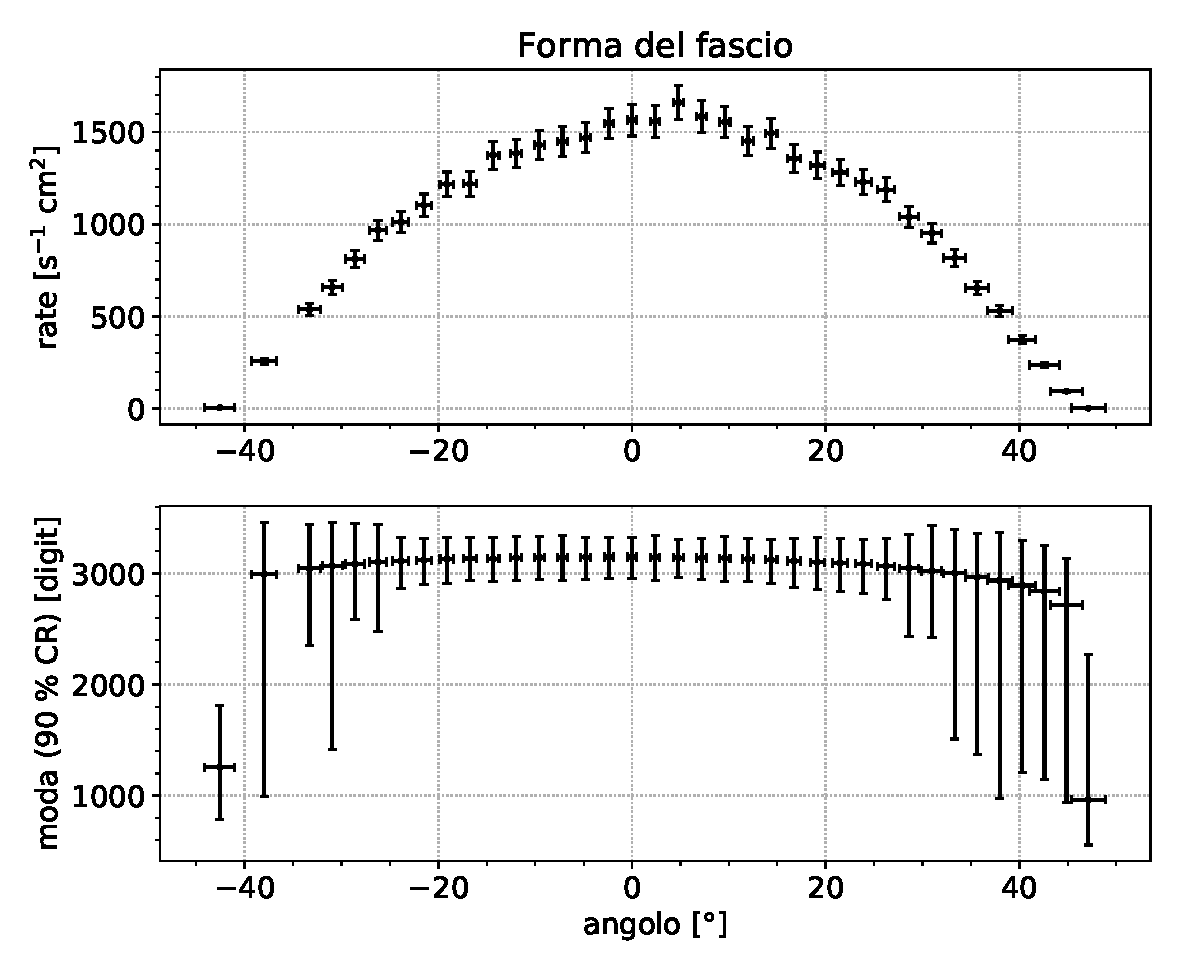
\includegraphics[width=30 em]{immagini/forma}
\caption{Grafico rappresentante la forma del fascio. Nel pannello superiore è presente l'estensione angolare del fascio estrapolata dai conteggi, in quello inferiore sono presenti le mode dei relativi istogrammi.}
\label{fig:forma}
\end{figure}

Useremo queste informazioni (se sarà necessario) nell'analizzare i dati sulla sezione d'urto.

\subsubsection{Collimatore da 5\! mm}

Analizziamo la forma del fascio con un collimatore da \SI{5}{mm} che ci dà un errore minore sull'angolo di incidenza delle particelle $\alpha$.
Con i dati presenti in \autoref{tab:coll5} abbiamo il grafico di \autoref{fig:coll5}.

In questo caso i conteggi sono non nulli soltanto nell'intervallo \SI{\mp10}{\degree}. La parte piatta al centro del grafico è dovuta all'effetto descritto nella sezione precedente (non corretto), ancora visibile con un'apertura di tale larghezza.

\begin{figure}[h]
\centering
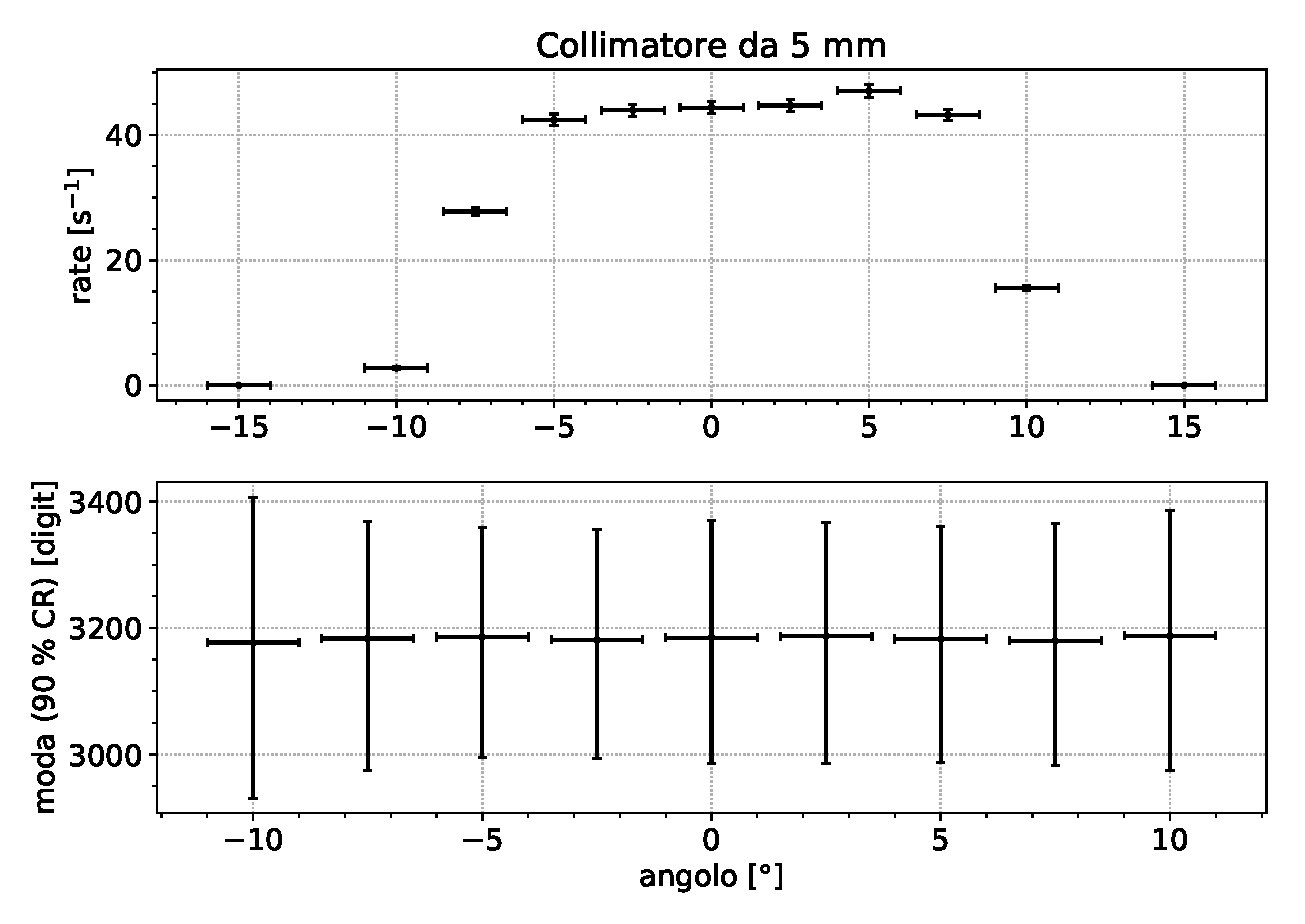
\includegraphics[width=30 em]{immagini/coll5}
\caption{Grafico del rate in funzione dell'angolo con il collimatore da 5\! mm.}
\label{fig:coll5}
\end{figure}

\subsubsection{Collimatore da 1\! mm}

Studiamo la forma del fascio con il collimatore da \SI1{mm} che ci permette di avere il più piccolo errore possibile sull'angolo di incidenza.
Di contro abbiamo un rate minore che nei casi precedenti.
I dati presenti in \autoref{tab:coll1} e \autoref{fig:coll1} sono stati analizzati come in precedenza.
Stavolta abbiamo conteggi solo in un intervallo di \SI{5}{\degree}.


\begin{figure}[h]
\centering
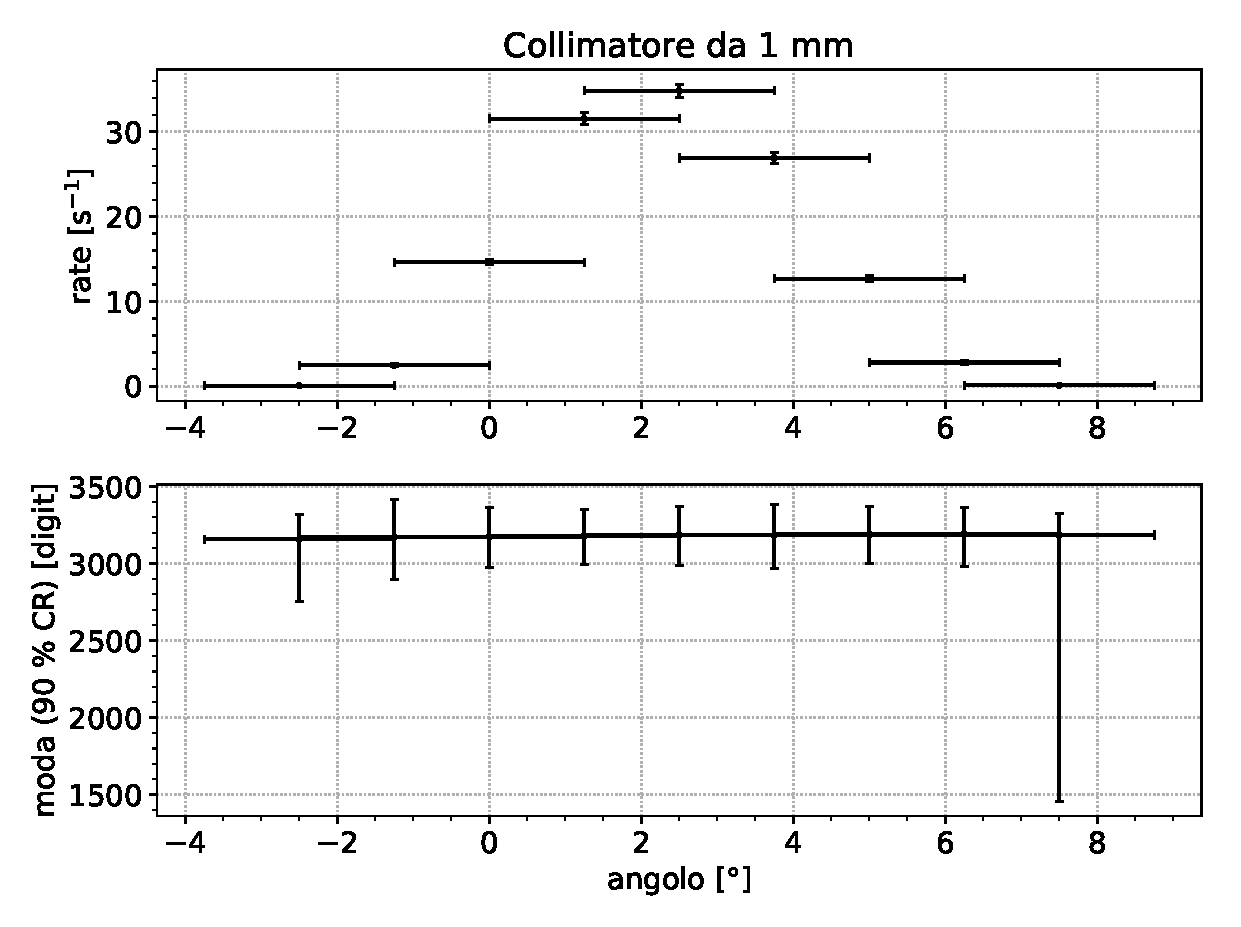
\includegraphics[width=30 em]{immagini/coll1}
\caption{Grafico del rate in funzione dell'angolo con il collimatore da 1\! mm.}
\label{fig:coll1}
\end{figure}

\subsubsection{Collimatore a croce}
\marginpar{questa sezione è particolarmente inutile, la toglierei (Bob)}
Cerchiamo infine di collimare il fascio il più possibile sovrapponendo 2 collimatori da \SI1{mm} di cui uno ruotato di \SI{90}{\degree} rispetto all'altro. In questo modo abbiamo una piccola finestra che seleziona le particelle sia verticalmente che orizzontalmente.
Prendiamo le misure in \autoref{tab:super} e guardiamo il grafico di \autoref{fig:super}.

\begin{figure}[h]
\centering
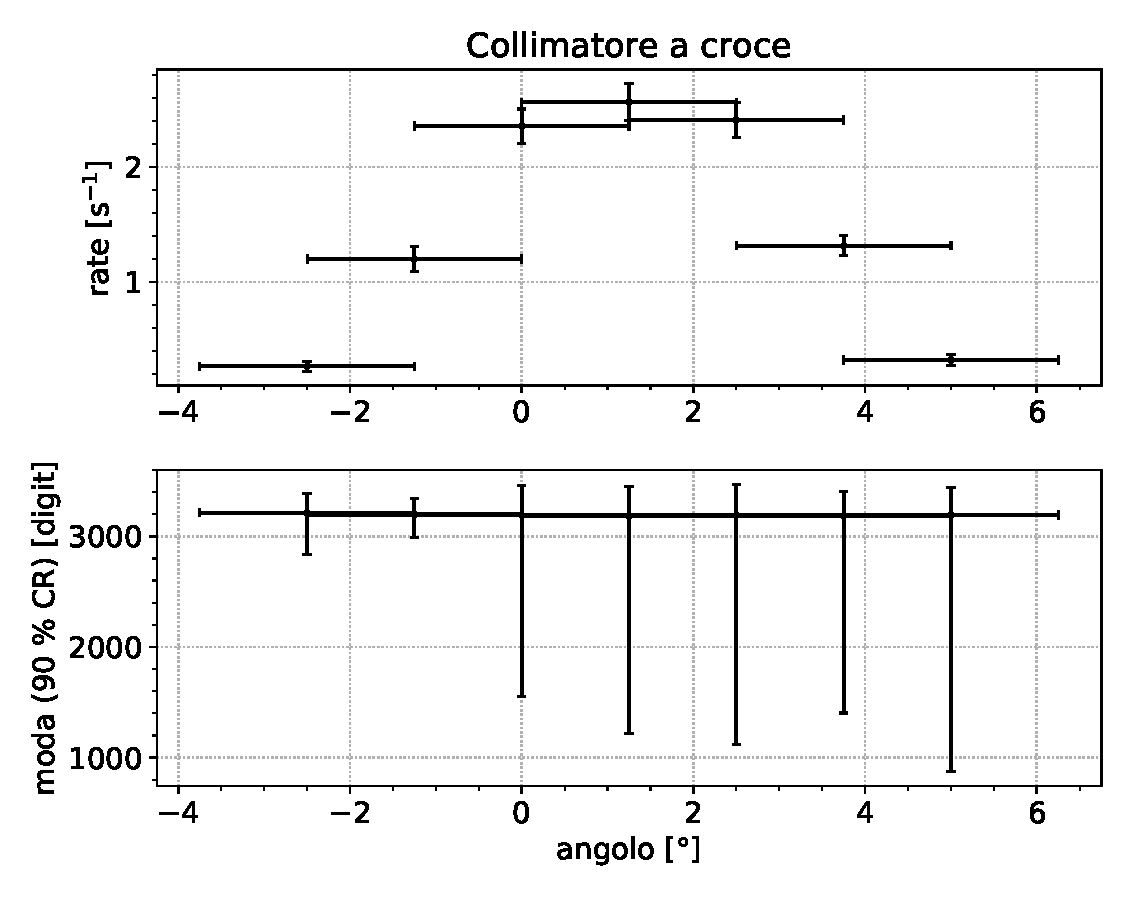
\includegraphics[width=30 em]{immagini/supercoll}
\caption{Grafico del rate in funzione dell'angolo con il collimatore a croce.}
\label{fig:super}
\end{figure}

Questa configurazione è ottimale per avere un fascio collimato, ma non la useremo a causa del rate incredibilmente basso.



